\documentclass[12pt,letterpaper]{article}
\usepackage{graphicx,textcomp}
\usepackage{natbib}
\usepackage{setspace}
\usepackage{fullpage}
\usepackage{color}
\usepackage[reqno]{amsmath}
\usepackage{amsthm}
\usepackage{fancyvrb}
\usepackage{amssymb,enumerate}
\usepackage[all]{xy}
\usepackage{endnotes}
\usepackage{lscape}
\newtheorem{com}{Comment}
\usepackage{float}
\usepackage{hyperref}
\newtheorem{lem} {Lemma}
\newtheorem{prop}{Proposition}
\newtheorem{thm}{Theorem}
\newtheorem{defn}{Definition}
\newtheorem{cor}{Corollary}
\newtheorem{obs}{Observation}
\usepackage[compact]{titlesec}
\usepackage{dcolumn}
\usepackage{tikz}
\usetikzlibrary{arrows}
\usepackage{multirow}
\usepackage{xcolor}
\newcolumntype{.}{D{.}{.}{-1}}
\newcolumntype{d}[1]{D{.}{.}{#1}}
\definecolor{light-gray}{gray}{0.65}
\usepackage{url}
\usepackage{listings}
\usepackage{color}

\definecolor{codegreen}{rgb}{0,0.6,0}
\definecolor{codegray}{rgb}{0.5,0.5,0.5}
\definecolor{codepurple}{rgb}{0.58,0,0.82}
\definecolor{backcolour}{rgb}{0.95,0.95,0.92}

\lstdefinestyle{mystyle}{
	backgroundcolor=\color{backcolour},   
	commentstyle=\color{codegreen},
	keywordstyle=\color{magenta},
	numberstyle=\tiny\color{codegray},
	stringstyle=\color{codepurple},
	basicstyle=\footnotesize,
	breakatwhitespace=false,         
	breaklines=true,                 
	captionpos=b,                    
	keepspaces=true,                 
	numbers=left,                    
	numbersep=5pt,                  
	showspaces=false,                
	showstringspaces=false,
	showtabs=false,                  
	tabsize=2
}
\lstset{style=mystyle}
\newcommand{\Sref}[1]{Section~\ref{#1}}
\newtheorem{hyp}{Hypothesis}


\title{\textbf{Replication:} \\Personal Economic Shocks and Public Opposition to Unauthorized Immigration}
\author{Daniel J. Hopkins\thanks{Department of Political Science, University of Pennsylvania, Philadelphia, PA, USA} \and Yotam Margalit\thanks{Department of Political Science, Tel Aviv University, Tel Aviv, Israel}\thanks{Department of Political Economy, King’s College London, London, UK} \and Omer Solodoch\thanks{Browne Center for International Politics, University of Pennsylvania, Philadelphia, PA, USA}\thanks{Department of International Relations, Hebrew University of Jerusalem, Jerusalem, Israel}}
\date{\small British Journal of Political Science (2023), page 1 of 9 \\
	doi:10.1017/S0007123423000261}

\begin{document}

\maketitle

\section*{Abstract (original research)}

Do negative economic shocks heighten public opposition to immigration, and through what mechanisms? Extant research suggests that economic circumstances and levels of labour market competition have little bearing on citizens’ immigration attitudes. Yet personal economic shocks have the potential to trigger the threatened, anti-immigration responses – possibly through channels other than labour market competition – that prior cross-sectional research has been unable to detect. To examine these propositions, we used a unique panel study which tracked a large, population-based sample of Americans between 2007 and 2020. We found that adverse economic shocks, especially job losses, spurred opposition to unauthorized immigration. However, such effects are not concentrated among those most likely to face labour market competition from unauthorized immigrants. Instead, they are concentrated among white male Americans. This evidence suggests that the respondents’ anti-immigration turn does not stem from economic concerns alone. Instead, personal experiences with the economy are refracted through salient socio-political lenses.\\
\\\textbf{Keywords:} immigration; unemployment; public opinion; panel data

\pagebreak
\section*{Replication objectives}
The key objectives of the replication is as follows:
\begin{itemize}
	\item Establish credibility to the researchers original work
	\item Learn how to perform various statistical analysis on primary data
	\item Add value to the research by making contributions
\end{itemize}
The researchers created a binary dependent variable to map whether respondent support deportation of unauthorised immigrants or not. The original variable captures responses on a 7-point scale ranging from 1 (‘Return illegal immigrants to their native countries’) to 7 (‘Create a pathway to U.S. citizenship for illegal immigrants’). As we can see, the original 7-point scale variable provides more food for thought and so, for the replication exercise, I will be using a multinomial ordered logit model and use this original variable to measure the effect.\\
When using a 7-point scale variable, the ordered multinomial model will help us understand how a unit change in independent variable is associated with the change in log odds on average for each one step jump in support of unauthorised immigrants.\\
\\As first step, the dependent variable is ordered and level "1" is set as the reference category using the following \texttt{R} code:
\lstinputlisting[language=R, firstline=162, lastline=164]{Shekhar Kedia_Script.R}  

\vspace*{.2cm}

\section*{Dataset}
A population-based panel of American respondents who were eighteen or older in 2008 was employed. Knowledge Networks (later GfK and then Ipsos) recruited panelists offline via address-based sampling or random-digit dialing. The first wave was administered in October 2007, and
the fifteenth wave in October 2020. However, it is important to note that the dependent variable was measured from 2012 onward.\\
\\The table below shows the key demographics of the respondents. We can see that the respondents in the latest October 2020 survey are quite similar to the respondents in the October 2012 survey in terms of demographics. The survey has 12 per cent Black, 11 per cent Hispanic, and about 71 per cent White people, with 38 per cent reporting a college degree.\\
\\The \texttt{R} code for producing the descriptive summary for both rounds of survey is:
\lstinputlisting[language=R, firstline=45, lastline=114]{Shekhar Kedia_Script.R}

\begin{center}
	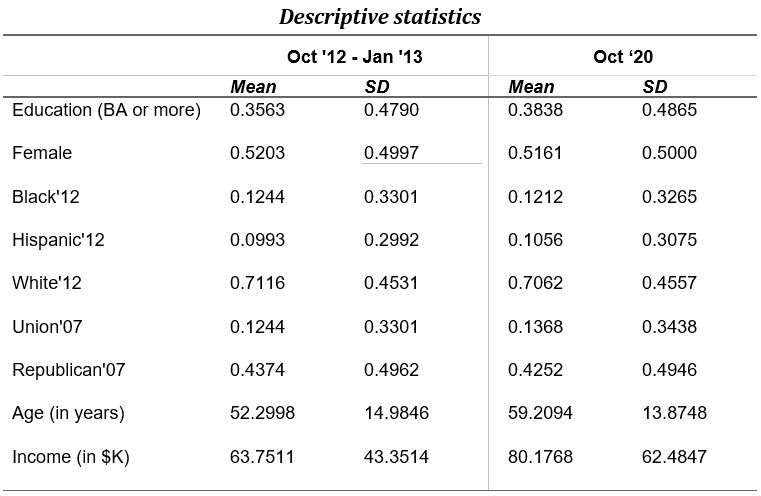
\includegraphics{Descriptive Stats.png}  
\end{center}
\textit{\textbf{N.B.:} The table output is formatted and inserted as image to reduce clutter and give a neat look to the document.}

\vspace*{.2cm}

\pagebreak
\section*{Results}
In this section, I will be first replicating the findings of the author and then running the multinomial ordered logit model with the 7-point scale dependent variable.\\
\\\textbf{Model: Unemployment and support for deportation of unauthorised migrants}
\lstinputlisting[language=R, firstline=118, lastline=145]{Shekhar Kedia_Script.R}
\textit{\textbf{N.B.:} The script is truncated and contains more information on table formatting which can be found in the \texttt{R} script file.}

\begin{center}
	\textbf{Table 1:}
	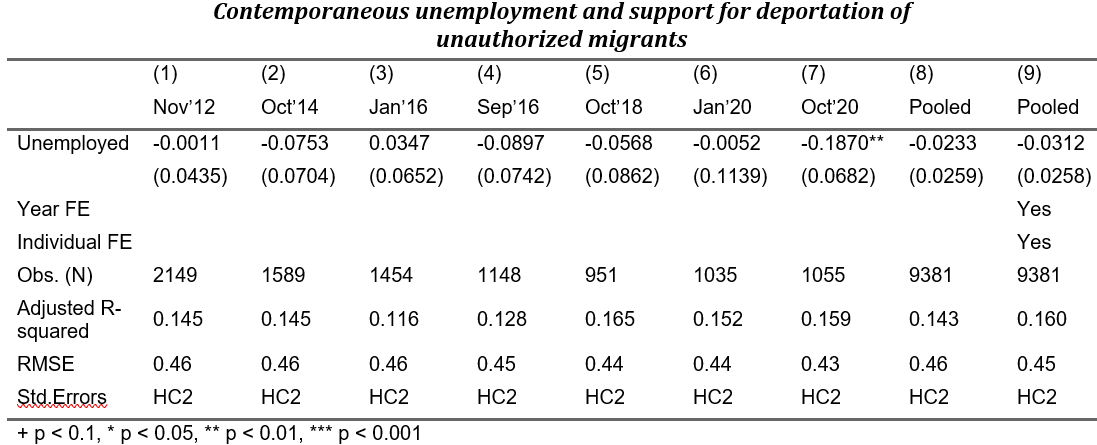
\includegraphics[scale=0.9]{Table 1.png}
\end{center}
\textit{\textbf{Notes:} Outcome variable is a binary indicator that equals 1 if the respondent supports deporting unauthorized migrants, and 0 otherwise. All regressions control for respondents’ age, race, gender, level of education, income employment status (retired, disabled or other), and partisanship (an indicator variable for Republicans). Robust standard errors in parentheses.}\\
\\From the above table we see that there is no evidence to suggest that if respondent is unemployed, it is associated with them supporting deportation of unauthorised migrants (for the full model).\\
\\Next, I run the multinomial ordered logit model with the 7-point scale dependent variable.
\lstinputlisting[language=R, firstline=166, lastline=175]{Shekhar Kedia_Script.R}  
\begin{Verbatim}
				Table 2:
	                   Value   Std. Error      t value p value
	UNEMPLOYED   0.196983424 0.0062094605    31.723114  0.0000
	RETIRED      0.149432095 0.0564906830     2.645252  0.0082
	DISABLED    -0.121698241 0.0278003426    -4.377581  0.0000
	OTHER_EMP    0.105875083 0.0730957009     1.448445  0.1475
	ppeducat     0.448982870 0.0296304055    15.152775  0.0000
	union0      -0.125712220 0.0552735429    -2.274365  0.0229
	white6      -0.248112956 0.0491833466    -5.044654  0.0000
	male        -0.201135932 0.0381265758    -5.275479  0.0000
	AGE          0.003473527 0.0023848264     1.456511  0.1453
	pre_party1  -1.162072214 0.0400357488   -29.025864  0.0000
	INCOME       0.001781918 0.0003965795     4.493217  0.0000
	Year         0.058865588 0.0001148059   512.740008  0.0000
	state       -0.001633945 0.0012222045    -1.336883  0.1813
	1|2        118.184158533 0.0112448075 10510.109544  0.0000
	2|3        118.660845411 0.0191759134  6188.015281  0.0000
	3|4        119.113187201 0.0232719513  5118.315431  0.0000
	4|5        119.991815895 0.0289024713  4151.610931  0.0000
	5|6        120.603579530 0.0323543872  3727.580396  0.0000
	6|7        121.257656034 0.0365344216  3318.997560  0.0000
\end{Verbatim}
We can see from the results that one unit change in \texttt{UNEMPLOYED} variable that is moving from "unemployed" to "employed" is associated with an increase of 0.197 log odds on average for a one step change of \texttt{path} variable which captures support for deportation on a 7-point scale ranging from 1 (‘Return illegal immigrants to their native countries’) to 7 (‘Create a pathway to U.S. citizenship for illegal immigrants’) holding all other covariates constant.\\
So, we find sufficient evidence to say that unemployed respondents oppose the deportation of unauthorised immigrants.\\
\\
\textbf{Model: Effect of economic shocks on support for deportation of unauthorised migrants}
\lstinputlisting[language=R, firstline=178, lastline=189]{Shekhar Kedia_Script.R}
\textit{\textbf{N.B.:} The script is truncated and contains more information on table formatting which can be found in the \texttt{R} script file.}

\begin{center}
	\textbf{Table 3:}
	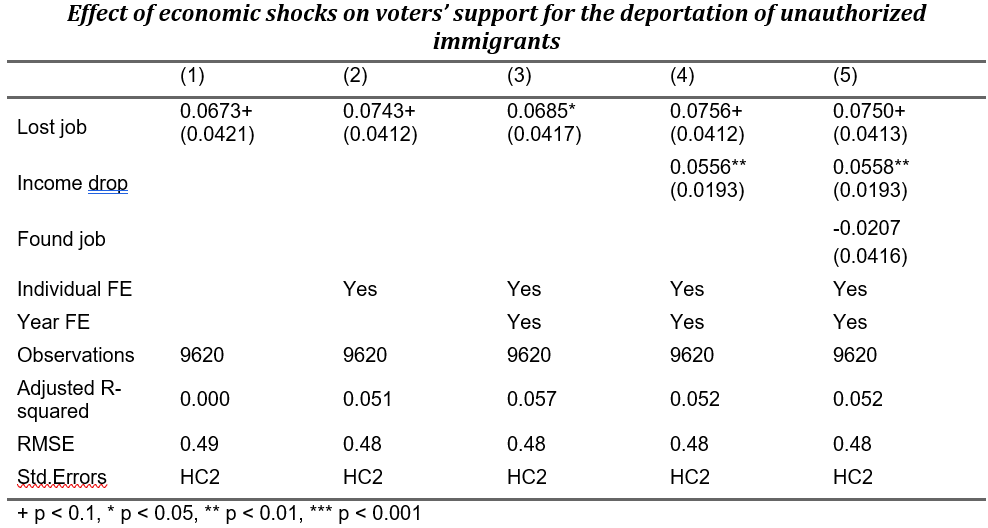
\includegraphics{Table 2.png} 
\end{center}
\textit{\textbf{Notes:} Outcome variable is a binary indicator that equals 1 if respondents support deporting unauthorized migrants and 0 otherwise. All regressions control for respondents’ level of education, level of income (logged), and employment status. Robust standard errors in parentheses.}\\
\\Across different model specifications we see that if respondent has lost job recently or experienced a drop in income (either personal or family), it affects opposition to unauthorised immigration.\\
\\Respondents who recently lost their job are 7.5 percentage points more supportive of deporting unauthorised immigrants. Again, a major income drop (of at least 25 per cent) is associated with a 5.5 percentage points increase in opposition to unauthorised immigration.\\
\\We also see that if the respondent has recently found a job, it is negatively associated with support for deporting authorised immigration. However, the coefficient is not statistically reliable.\\
\pagebreak
\\Next, I run the multinomial ordered logit model with the 7-point scale dependent variable.
\lstinputlisting[language=R, firstline=208, lastline=217]{Shekhar Kedia_Script.R}
\begin{Verbatim}
				Table 4:
                         Value  Std. Error    t value p value
LOST_JOB          -0.213567659 0.151907476 -1.4059062  0.1598
income_shock2     -0.207933736 0.069856838 -2.9765695  0.0029
FOUND_JOB          0.133809587 0.153516189  0.8716318  0.3834
RETIRED            0.246179562 0.044447214  5.5386950  0.0000
DISABLED          -0.034218629 0.085938449 -0.3981760  0.6905
OTHER_EMP          0.029195483 0.076193952  0.3831732  0.7016
factor(ppeducat)2  0.289677605 0.105699855  2.7405677  0.0061
factor(ppeducat)3  0.749595032 0.108924429  6.8817899  0.0000
factor(ppeducat)4  1.379924562 0.108846389 12.6777247  0.0000
logINCOME          0.008965511 0.023801613  0.3766766  0.7064
state             -0.003784855 0.001160226 -3.2621718  0.0011
1|2               -0.428223520 0.142333975 -3.0085826  0.0026
2|3                0.017343994 0.142232843  0.1219409  0.9029
3|4                0.426003191 0.142231108  2.9951478  0.0027
4|5                1.220687717 0.142668735  8.5560983  0.0000
5|6                1.778897021 0.143251141 12.4180304  0.0000
6|7                2.383304486 0.144104814 16.5386875  0.0000
\end{Verbatim}
We can see from the results that one unit change in \texttt{income\_shock2} variable that is experiencing a major income drop (of at least 25 per cent) is associated with a decrease of 0.207 log odds on average for a one step change of \texttt{path} variable which captures support for deportation on a 7-point scale ranging from 1 (‘Return illegal immigrants to their native countries’) to 7 (‘Create a pathway to U.S. citizenship for illegal immigrants’) holding all other covariates constant.\\
\\The coefficient for recent \texttt{LOST\_JOB} and \texttt{FOUND\_JOB} is not statistically reliable.\\

\pagebreak

\textbf{Model: Effect heterogeneity by respondent characteristics}
\lstinputlisting[language=R, firstline=220, lastline=242]{Shekhar Kedia_Script.R}
\textit{\textbf{N.B.:} The script is truncated and contains more information on table formatting which can be found in the \texttt{R} script file.}
\pagebreak
\begin{center}
	\textbf{Table 5:}
	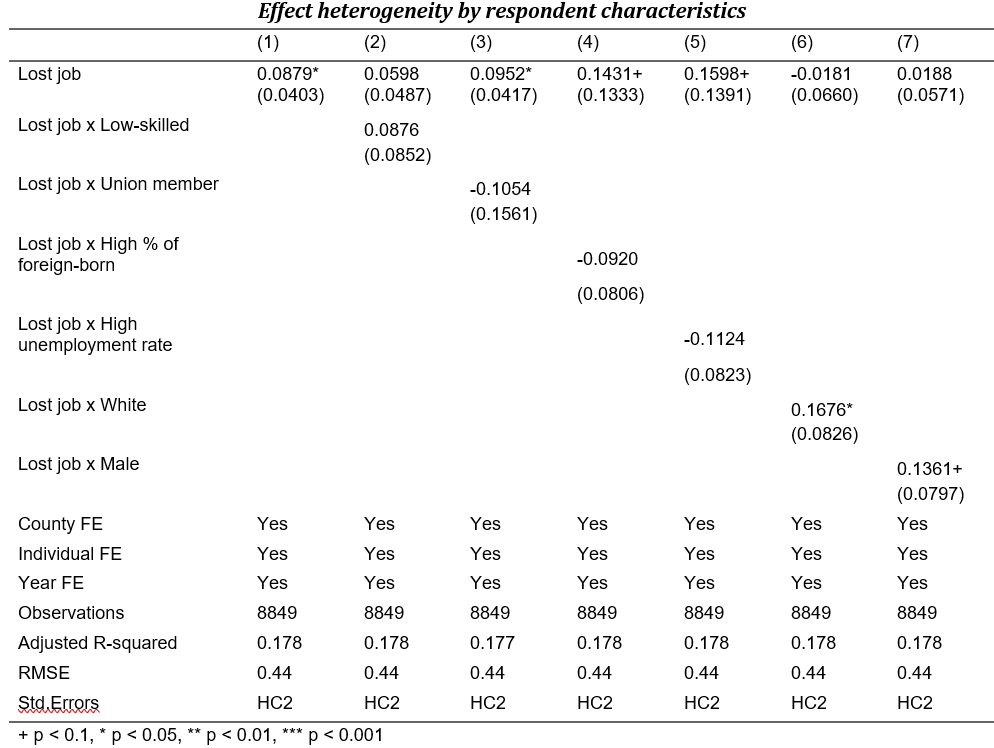
\includegraphics{Heterogeneity.png} 
\end{center}
\textit{\textbf{Notes:} Outcome variable is a binary indicator that equals 1 if the respondent supports deporting unauthorized migrants, and 0 otherwise. The linear probability models in columns 2–7 interact with unemployment shocks with indicator variables denoting the different groups of respondents. All regressions control for the constitutive terms of the interaction with job loss and age, income, employment status (retired, disabled or other) and partisanship. Robust standard errors in parentheses.}\\
\\We can see from the above table that there is no evidence of heterogeneous effects across respondents (who recently lost their jobs) differentiated by skill level or union membership. Also, no evidence is found in case of such respondents belonging to counties with higher percentage of foreign-born or unemployment rate. However, we do find some evidence that white respondents who have recently lost their jobs are 16.76 percentage points more opposed to unauthorised immigration. Furthermore, male respondents who have recently lost their jobs are 13.61 percentage points more opposed to unauthorised immigration. 

\pagebreak

\section*{Conclusion}
From the research, we find that labour market factors like unemployment rate and counties with high proportion of foreign-born do not affect opposition towards unauthorised immigrants. However personal economic factors like recent job loss or income shock (of at least 25\%) is associated with negative sentiment towards unauthorised immigrants and support their deportation.\\
\\Furthermore, from the heterogeneity model we observe that white respondents and male respondents who have faced recent job loss are more likely to support deportation of unauthorised immigrants.\\
\\On doing the replication of key results, I was able to confirm similar results as originally reported by the authors.\\
Moreover, as part of my contribution to the research, when I used the original 7-point scale dependent variable, I was able to find that majority of the trends remained the same (as with the authors work), just that the effects of \texttt{UNEMPLOYED} variable was found to be different (in Model 1).

\vspace*{.2cm}

\section*{Replication limitations}
The authors used STATA to run the regression models. However, as part of my academic requirement, I had to use \texttt{R} for analysis. The original codes were therefore, rewritten in \texttt{R} for the replication exercise. I notice that while the broad trends and estimates are unchanged, there is marginal change in the estimation of standard errors.\\
\\The replication gave me a good opportunity to brush up my knowledge on STATA and implement same analysis in \texttt{R}.

\end{document}